

%%%%%%%%%%%%%%%%%%%%%%%%%%%%%%%%%%%

\begin{frame}
\frametitle{Filtros de fase 0 - I }

\vspace{-0.2cm}



\begin{itemize}
\footnotesize
\item Un filtro de de fase 0 es aquel que tiene una $H(e^{jw})$ real y no negativa.

\visible<2->{

\item Esto implica que no modifica la fase de la señal de entrada en la banda de paso.
}

\visible<3->{

\item Se puede implementar como  $H(z)=F(z)F(z^{-1})$, donde  F(z) es un sistema que no tiene polos sobre el círculo unidad. 

}

\visible<4->{

\item Por construcción es un filtro de fase 0:

$H(e^{jw})\!=H(z=e^{jw})=F(e^{jw})F(e^{-jw})=|F(e^{jw})|^2$, que es un número positivo real.

}

\visible<5->{

\item Si z es un polo (o cero) del sistema su inversa también lo es. Por lo tanto se colocan con una simetría especular respecto al circulo unidad. 
}

\visible<6->{


\item Este hecho hace que el sistema sea inestable, y que por lo tanto no se pueda aplicar directamente a una señal. 
}

\visible<7->{

\item Sin embargo, si se puede aplicar a una señal de longitud finita:

\begin{columns}[T]
\begin{column}{4cm}

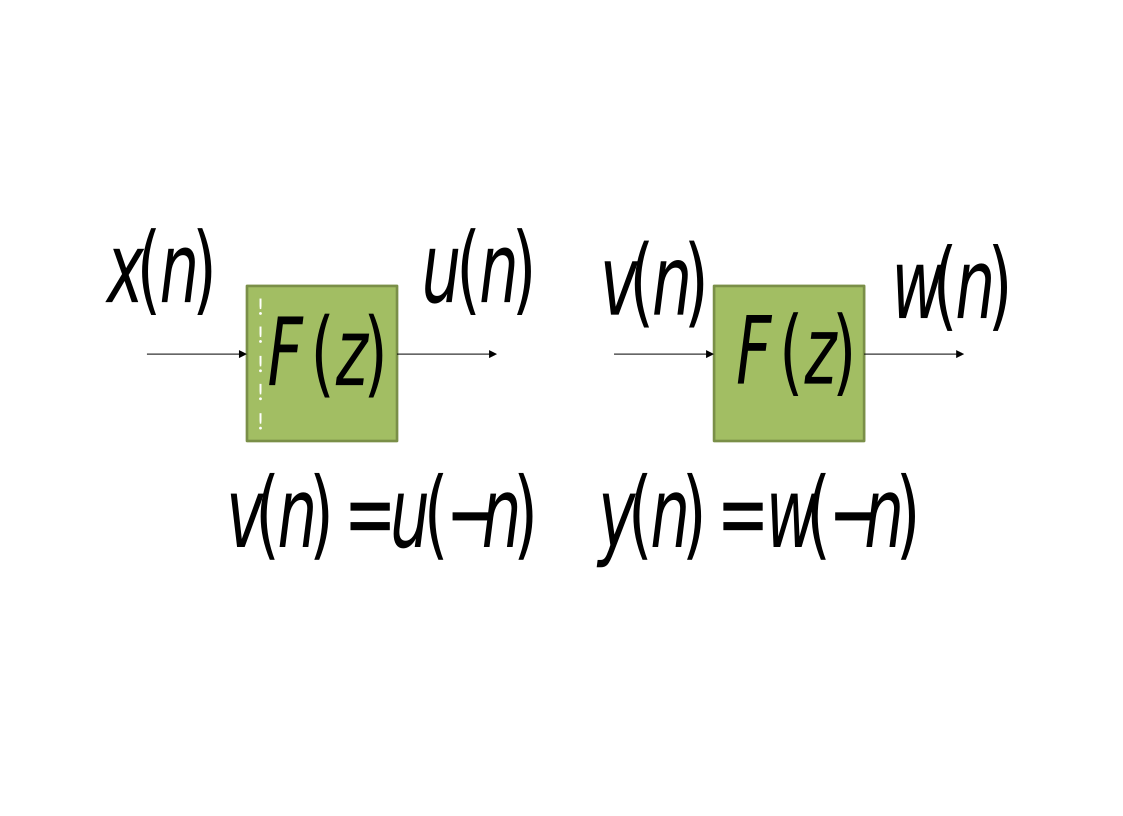
\includegraphics[trim=4cm 1cm 4cm 1cm,width=4cm]{Figures/FiltroFase0}
\end{column}
\begin{column}{4cm}

$Y(e^{jw})=W^*(e^{jw})=F^*(e^{jw})V^*(e^{jw})=F^*(e^{jw})U(e^{jw})=F^*(e^{jw})F(e^{jw})X(e^{jw})=|F(e^{jw})|^2X(e^{jw})$
\end{column}
\end{columns}
}



\visible<8->{
\item La orden de Matlab \color{blue}\texttt{y=filtfilt(Fnumz,Fdenz,x)}\color{black} permite realizar el filtrado con el procedimiento anteriormente escrito.
}


\end{itemize}
\end{frame}

\begin{frame}
\frametitle{Ejemplo Filtro Fase 0 - II}
\footnotesize

\begin{itemize}

\item Implementación a través de la $F(z)$: $H(z)=F(z)F(z^{-1})$

\hspace{4.8cm} $H(e^{jw})=|F(e^{jw})|^2$

\visible<2->{

\item El hecho de que en $H(z)$ aparezca un polo y su inversa, hace que el numerador y el denominador sean productos de polinomios   $B(z)=\sum_{l=0}^N b_l(z^l+z^{-l})$

\color{gray}

Ejemplo: $(z-a)(z^{-1}-a)=(1-az-az^{-1}+a^2)=(1+a^2)+a(z^1+z^{-1})$

\color{black}
}

\visible<3->{


\item Una forma habitual de diseñar este tipo de filtros es definir la $H(e^{jw})$ deseada, y obtener a continuación la F(z) aprovechando la propiedad de que la localización de los ceros y polos con simetría especular hace que en la H(z) aparezcan productos de polinomios $B(z)=\sum_{l=0}^N b_l(z^l+z^{-l})$, y que esto a su vez implica que en la respuesta en frecuencia tendremos términos del tipo $B(e^{jw})=\sum_{l=0}^N b_l(e^{jwl}+e^{-jwl})=b_0+\sum_{l=0}^N 2b_lcos(wl)$


\item A continuación veremos con un ejemplo la forma de proceder.
}

\end{itemize}
\end{frame}

\begin{frame}
\frametitle{Ejemplo Filtro Fase 0}
\footnotesize

\color{olivegreen} Calcular la F(z) de un filtro de fase 0 con  $H(e^{jw})=\frac{4(1.09+0.6cos(w))(1.16-0,8cos(w))}{(1.04-0.4cos(w))(1.25+cos(w))}$




\color{gray}

\vspace{0.2cm}

$H(e^{jw})=|F(e^{jw})|^2=\frac{4(1.09+0.3(e^{jw}+e^{-jw}))(1.16-0,4(e^{jw}+e^{-jw}))}{(1.04-0.2(e^{jw}+e^{-jw}))(1.25+0.5(e^{jw}+e^{-jw}))}$

\vspace{0.2cm}

$F(z)F(z^{-1})=\frac{4(1.09+0.3(z+z^{-1}))(1.16-0,4(z+z^{-1}))}{(1.04-0.2(z+z^{-1}))(1.25+0.5(z+z^{-1}))}=$

\vspace{0.2cm}

$F(z)F(z^{-1})=\frac{4(1+0.3z)(1+0.3z^{-1})(1-0.4z)(1-0.4z^{-1})}{(1-0.2z)(1-0.2z^{-1})(1+0.5z)(1+0.5z^{-1})}$

\vspace{0.2cm}

$F(z)=\frac{2(1+0.3z)(1-0.4z)}{(1-0.2z)(1+0.5z)}$


\end{frame}
